
\chapter{A Combinatorial Miscellany}


%\section{Domino Tilings}


%\section{Permutations}

\section{Perfect Matchings and Pfaffian Orientations}
Refer to \href{https://youtu.be/ydCWu6aiAxE?si=v91XmPDjM3qkfGKw}{https://youtu.be/ydCWu6aiAxE?si=v91XmPDjM3qkfGKw}. 
\section{Graphs and Trees}
We start with a standard result on graphs.
\begin{theorem}
    Let $G$ be a simple, connected graph on $n$ vertices. Then the following are equivalent.
    \begin{enumerate}
        \item $G$ is minimally connected.
        \item $G$ has $n-1$ edges.
        \item $G$ has no cycles.
    \end{enumerate}
    \label{t:G&T_Main}
\end{theorem}
\begin{proof}
If $G$ is minimally connected, then removing any edge of $G$ would disconnect it. This means that each edge of $G$ is a bridge. Since G is connected, it must have at least $n-1$ edges. If G had more than $n-1$ edges, then removing any additional edge would not disconnect $G$, contradicting the minimality assumption. Therefore, $G$ must have exactly $n-1$ edges. This proves that $(1)\implies (2)$. If G has $n-1$ edges and $n$ vertices, then it is a tree. Trees are acyclic by definition, so $G$ has no cycles. This proves $(2)\implies (3)$. Finally, if G has no cycles, then it is a tree. Trees are minimally connected, meaning that removing any edge disconnects the graph. Therefore, $G$ is minimally connected. This proves $(3)\implies (1)$. Having formed a loop of implications, we are done.
\end{proof}
Recall the following definitions. Graphs satisfying any one of the properties in \cref{t:G&T_Main} are called trees. Additionally, graphs whose connected components are trees are called forests. More importantly, a tree on $n$ vertices is called a labeled tree if each vertex gets a label from the set $[n]$. 
\par
With this background at hand, we are interested in counting $T_n$, the number of labeled trees on $n$ vertices. From the figure below it is clear that $T_1,T_2,T_3$ and $T_4$ are $1,1,3$ and $16$. One might guess that $T_n=n^{n-2}$. In fact this is precisely what we want to prove.
\begin{figure}[H]
    \centering
    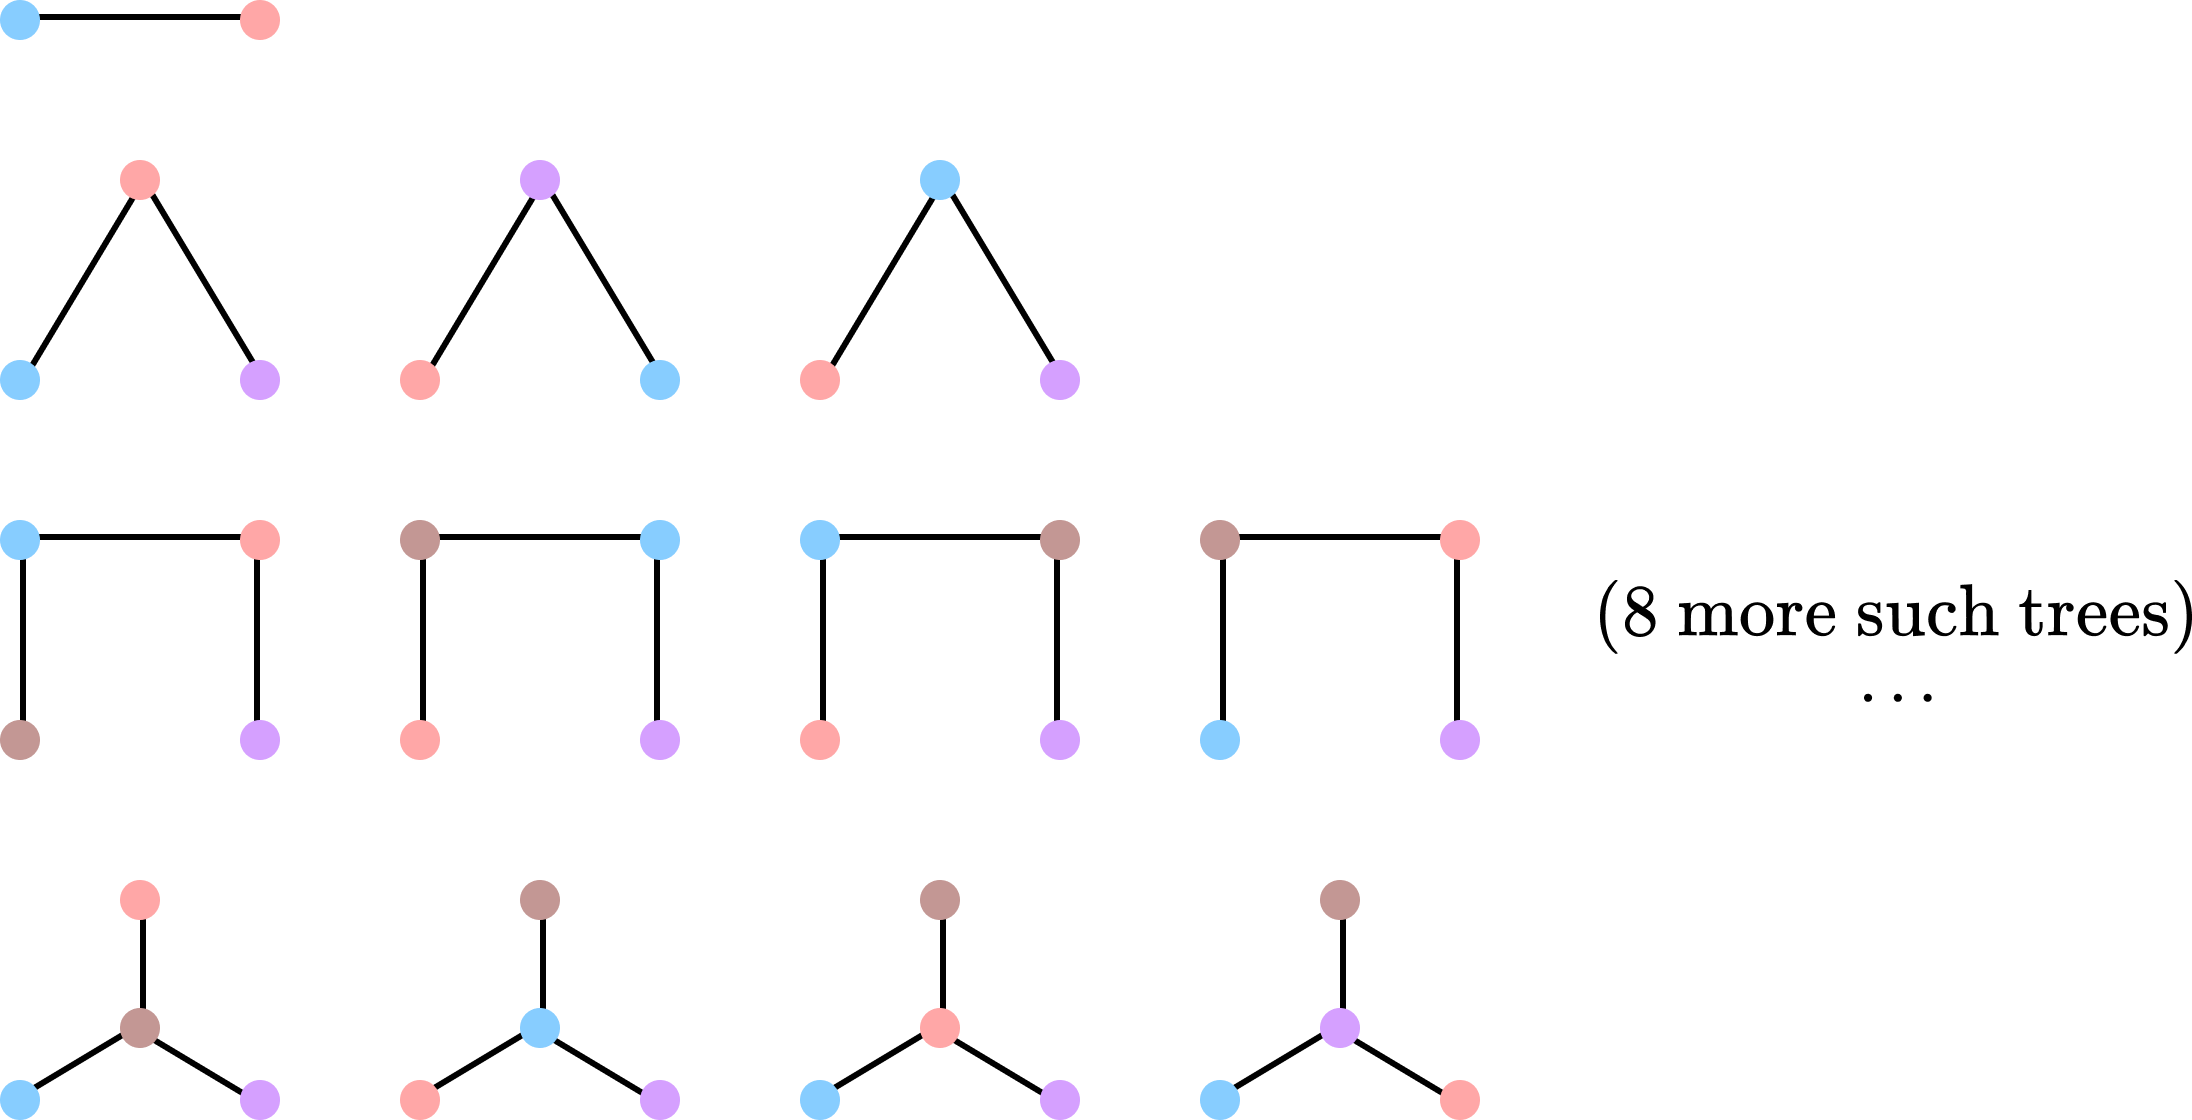
\includegraphics[width=0.9\linewidth]{Images/Figure29.png}
    \caption{}
    \label{f:Cayley Trees}
\end{figure}

\begin{theorem}[Cayley's Formula]
If $T_n$ denotes the number of labeled trees on $n$ vertices, then
    \[
    T_n = n^{n-2}.
    \]
    \label{t:Cayley's Formula}
\end{theorem}
\begin{proof}
Let $A=[k]$ be a set of vertices. Let $T_{n,k}$ count the number of labeled forests on $[n]$ consisting of $k$ trees where the vertices of $A$ appear in different trees. Let $F$ be a forest in this setting.
\begin{figure}[H]
    \centering
    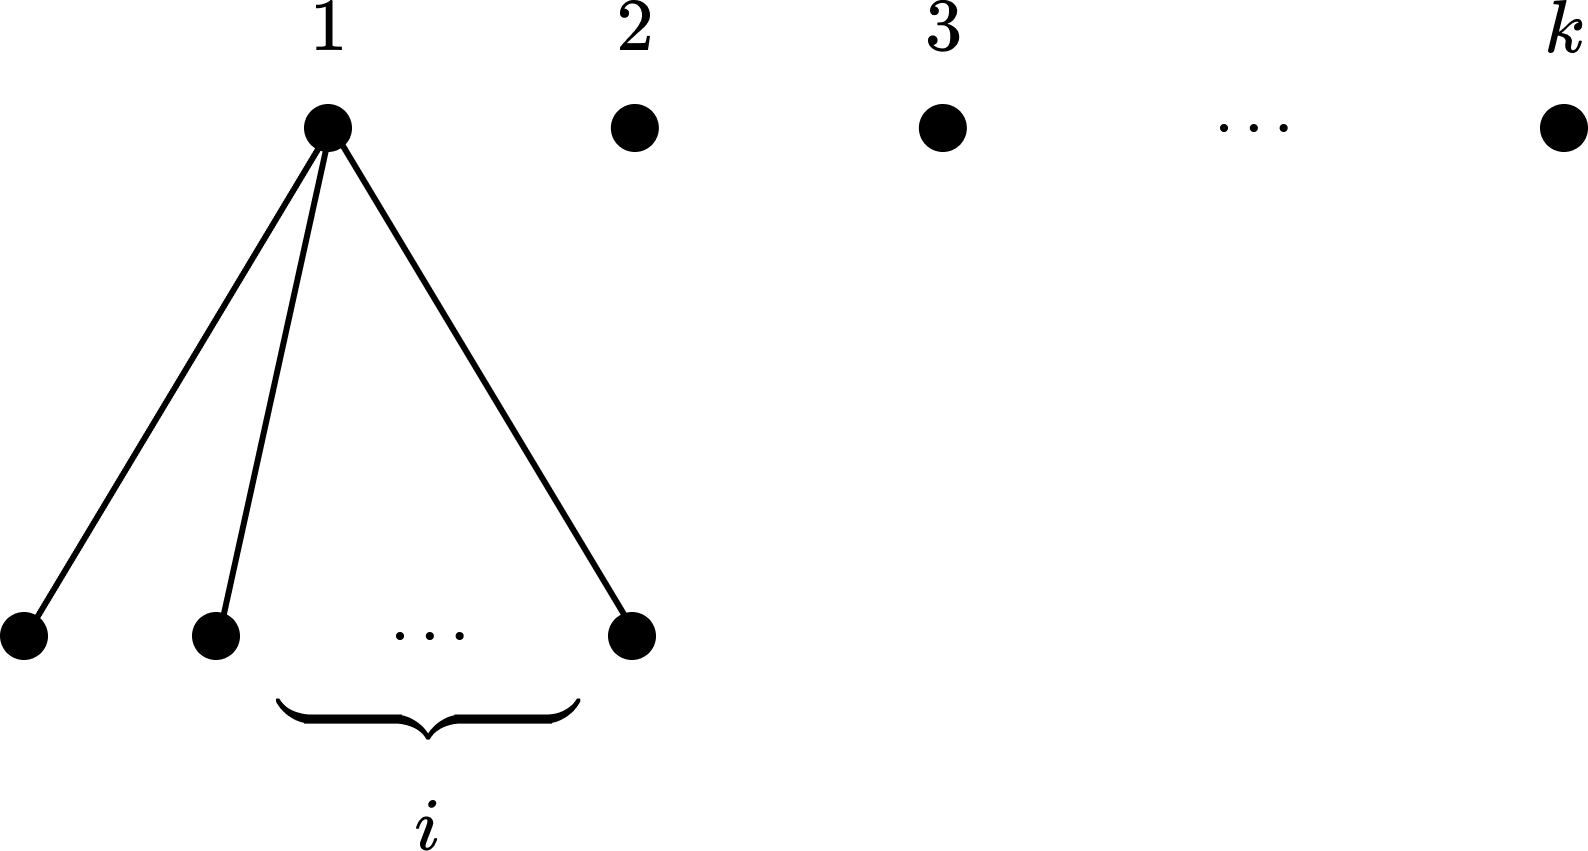
\includegraphics[width=0.5\linewidth]{Images/Figure30.png}
    \caption{}
    \label{f:CTProof}
\end{figure}
As is clear by \cref{f:CTProof}, if $1$ is adjacent to $i$ vertices, deleting it, the $i$ neighbors together with $2,\ldots,k$ yield one vertex each in the components of a forest that consists of $k-1+i$ trees. Since $F$ can also be constructed by fixing $i$, then choosing the $i$ neighbors of $1$ and then the forest $F\backslash \{1\}$ gives \[
T_{n,k} = \sum_{i=0}^{n-k}\binom{n-k}{i}T_{n-1,k-1+i}
\]
for all choices of $n\geq k\geq 1$ where $T_{0,0}=1$ and $T_{n,0}=0$ as expected. By induction and the expression for $T_{n,k}$ which we have found, it follows that
\begin{align*}
    T_{n,k}&= \sum_{i=0}^{n-k}\binom{n-k}{i}(k-1+i)(n-1)^{n-1-k-i} \\
    &= \sum_{i=0}^{n-k}(n-1)^i-\sum_{i=1}^{n-k}\binom{n-k}{i}i(n-1)^{i-1} \\
    &= n^{n-k}-(n-k)\sum_{i=0}^{n-1-k}\binom{n-1-k}{i}(n-1)^i \\
    &= n^{n-k}-(n-k)n^{n-1-k} \\
    &= kn^{n-1-k}.
\end{align*}
Setting $k\to 1$ gives us the required result.
\end{proof}
\begin{theorem}
The number of rooted forests on $[n]$ is $(n+1)^{n-1}$.
\end{theorem}
\begin{proof}
The proof follows from the following observation. For any rooted forest with \( n \) vertices, add a new vertex \( v \) and connect it to all the roots as their parent. This forms a tree with \( n + 1 \) vertices. Conversely, for any tree with \( n + 1 \) vertices, where one vertex is labeled \( v \), remove \( v \) along with its edges. The resulting structure is a rooted forest, with the former children of \( v \) serving as the roots.
\end{proof}
We conclude this section with a result whose proof we shall omit but see \cref{t:Cayley's Formula} as a consequence of. 
\begin{theorem}
    The number of rooted forests on $[n]$ with $k$ components is \[
    \binom{n-1}{k-1}n^{n-k}.
    \]
\end{theorem}
Notice how setting $k\to 1$ and multiplying the result by $n$ (to account for the $n$ choices of roots) gives \cref{t:Cayley's Formula} back. 
\section{Permutations Revisited}
We are interested in counting \( P_n \), the number of permutations on \([n]\) that can be generated using a single stack. We start by computing $P_n$ by hand for $n=1,2$ and $3$. When $n=1$, we can push $1$ on to the empty stack and pop it immediately. The stack is now empty, and there are no more input values. So we are done and the output is the permutation $(1)$. Next, when $n=2$, we have two possible permutations, $(12)$ and $(21)$. To obtain the permutation $(12)$, first push $1$ onto the stack, then pop it, then push $2$ onto the stack and then pop it. To obtain the permutation $(21)$, first push $1$ onto the stack, then push $2$, then pop $2$, and then pop $1$. Similarly, the permutations $(123),(132),(213),(231)$ and $(321)$ are obtainable. One might (correctly) guess from here one that this is the sequence of Catalan numbers. What follows is a proof of the same.
\begin{proof}
To this end, let \( i \) denote the position of the element \( 1 \) in a valid permutation produced by the stack, where \( 1 \leq i \leq n \). Then, \( P_{i-1} \) counts the number of valid permutations with \( i-1 \) elements to the left of \( 1 \), and \( P_{n-i-1} \) counts the number of valid permutations with \( n-i-1 \) elements to the right of \( 1 \). If we set \( P_0 = 1 \), then by the multiplication and addition principles, we obtain the recurrence
\[
P_n = \sum_{i=1}^n P_{i-1} P_{n-i-1},
\]
which, more explicitly is written as 
\[
P_n = P_0 P_{n-1} + P_1 P_{n-2} + \cdots + P_{n-1} P_0.
\]
Recall how this is precisely the recurrence relation we derived in \cref{t:segner}. Therefore, \( P_n = C_n \) for all \( n \geq 0 \), where \( C_n \) denotes the \( n \)-th Catalan number.
\end{proof}
\endinput
